\documentclass[10pt]{report}
\usepackage[headings]{fullpage}
\usepackage{scribe-hw}

\usepackage{amsfonts}
\usepackage{amssymb}
\usepackage{amsmath}
\usepackage{epsfig}
\usepackage{graphicx}
\usepackage{pstricks,pst-plot}
\usepackage{hyperref}

\def\F{{\cal F}}
\def\X{{\cal X}}
\def\Y{{\cal Y}}
\def\Z{{\cal Z}}
\def\P{{\mathbb P}}
\def\R{{\mathbb R}}
\def\E{{\mathbb E}}
\def\bZ{{\mathbb Z}}
\def\darkred{\color{red!70!black}}
\def\darkgreen{\color{green!60!black}}
\def\learn{{\mbox{LEARN}}}
\def\err{{\mbox{err}}}
\def\bI{{\tilde{I}}}
\def\dis{{\mbox{DIS}}}
\def\bR{{\mathbb R}}
\def\R{{\mathbb R}}
\def\eps{{\epsilon}}
\def\E{{\mathbb E}}
\def\epso{{\epsilon_o}}
\def\nicered{{\color{red!70!black}}}
\def\pr{{\mbox{\rm Pr}}}
\usepackage[most]{tcolorbox}
\newtcolorbox[]{solution}[1][]{%
    breakable,
    enhanced,
    colback=white,
    title=Solution,
    #1
}

\begin{document}

\course{CSE 151}
\coursetitle{Machine learning}
\semester{Fall 2019}
\lecturer{}
\scribe{}
\lecturenumber{3}
\lecturetopic{Homework}
\maketitle

\noindent
{\bf Submission instructions:} 
\begin{itemize}
\item If a problem asks for a numerical answer, you need only provide this answer. There is no need to show your work, unless you would like to.
\item Please type up your solutions. We suggest using an online latex editor like www.overleaf.com. We recommend you clone the provided read-only Overleaf project, and simply enter your solutions into the latex file.
\item Upload the PDF file for your homework to Gradescope by 11:59pm on {\bf Tuesday Dec 3}.
\item {\bf Please include your code for the problem as part of your submission on Gradescope.}
\end{itemize}

\vspace{.1in}

\begin{enumerate}

\item An SVM classifier is learned for a data set in $\R^2$. It is given by $w = (3,4)$ and $b = -12$ (or, equivalently, $w = (3,4,-12)$ where the last feature is the bias feature). 
\begin{enumerate}
\item[(a)] Draw the decision boundary, making sure to clearly indicate where it intersects the axes.
\item[(b)] Draw the $w \cdot x + b = 1$ and $w \cdot x + b = -1$ boundaries, also clearly marking where they intersect the axes.
\item[(c)] What is the margin of this classifier?
\item[(d)] How would the point $(2,2)$ be classified?
\item[(e)] It turns out that the data set has two distinct support vectors of the form $(1,?)$. What are they?
\end{enumerate}
\begin{solution}

% Write your solution here
\end{solution}

\item Consider the following small data set in $\R^2$:
\begin{itemize}
\item Points $(1,2), (2,1), (2,3), (3,2)$ have label $-1$.
\item Points $(4,5), (5,4), (5,6), (6,5)$ have label $+1$.
\end{itemize}
Now, suppose (hard margin) SVM is run on this data.
\begin{enumerate}
\item[(a)] Sketch the resulting decision boundary.
\item[(b)] What is the (numerical value of the) margin, exactly?
\item[(c)] What are $w$ and $b$, exactly? 
\end{enumerate}
\begin{solution}
% Write your solution here
\end{solution}

\item {\it Support vectors.} The picture below shows the decision boundary obtained upon running soft-margin SVM on a small data set of blue squares and red circles. The dotted lines show the $+1$ and $-1$ level-sets of the classifier's scoring function (i.e. $w^\top x + b = 1$ and $w^\top x + b = -1$).

\begin{center}
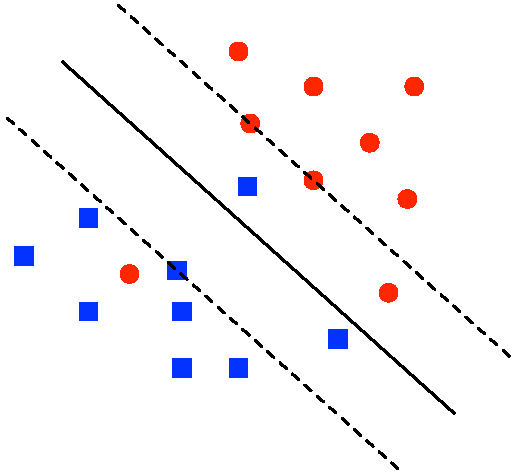
\includegraphics[width=2in]{support-vectors.pdf}
\end{center}

\begin{enumerate}
\item[(a)] Copy this figure (``support-vectors.pdf'') and mark the support vectors. For each, indicate the approximate value ($0$ or $> 0$) of the corresponding slack variable.
\item[(b)] Suppose the factor $C$ in the soft-margin SVM optimization problem were increased. Would you expect the margin to increase or decrease?
\end{enumerate}
\begin{solution}
    \begin{enumerate}
        \item
        \item expect the margin to decrease
    \end{enumerate}
% Write your solution here
\end{solution}

\item The dual form of the Perceptron algorithm is used to learn a binary classifier, based on $n$ training points. It converges after $k$ updates, and returns a vector $\alpha$ and a number $b$. For each of the following statements, indicate whether it is {\bf necessarily true} or {\bf possibly false}, and give a brief justification.
\begin{enumerate}
\item Each $\alpha_i$ is either 0 or 1.
\item $\sum_i \alpha_i = k$.
\item $\alpha$ has at most $k$ nonzero coordinates.
\item The training data must be linearly separable.
\end{enumerate}
\begin{solution}
    \begin{enumerate}
        \item possibly false
        \item necessarily true
        \item necessarily true
        \item necessarily true
    \end{enumerate}
% Write your solution here
\end{solution}

\item Suppose you are given a dataset with four points and two classes. First plot these points for yourself, and convince yourself that any linear classifier will be unable to classify all 4 points correctly. We have drawn you a simple 1 hidden layer MLP, with the 2 inputs ($X_1, X_2$), 2 hidden nodes ($H_1, H_2$), 2 bias features ($B^1, B^2$), and one output. All parameters names are listed in the table as well as illustrated on the figure: $W^L_{ij}$ is the weight that connects node i in layer L to node j in layer L+1. Assume that the sign activation function (i.e. returning +1 if input is positive, and -1 otherwise) is used at each node, except for the output node. For the output node, assume the logistic function is used to produce $P(y=1|x)$. Write down a setting of all parameters (weights) for this MLP that will perfect classify the training set.

\begin{center}
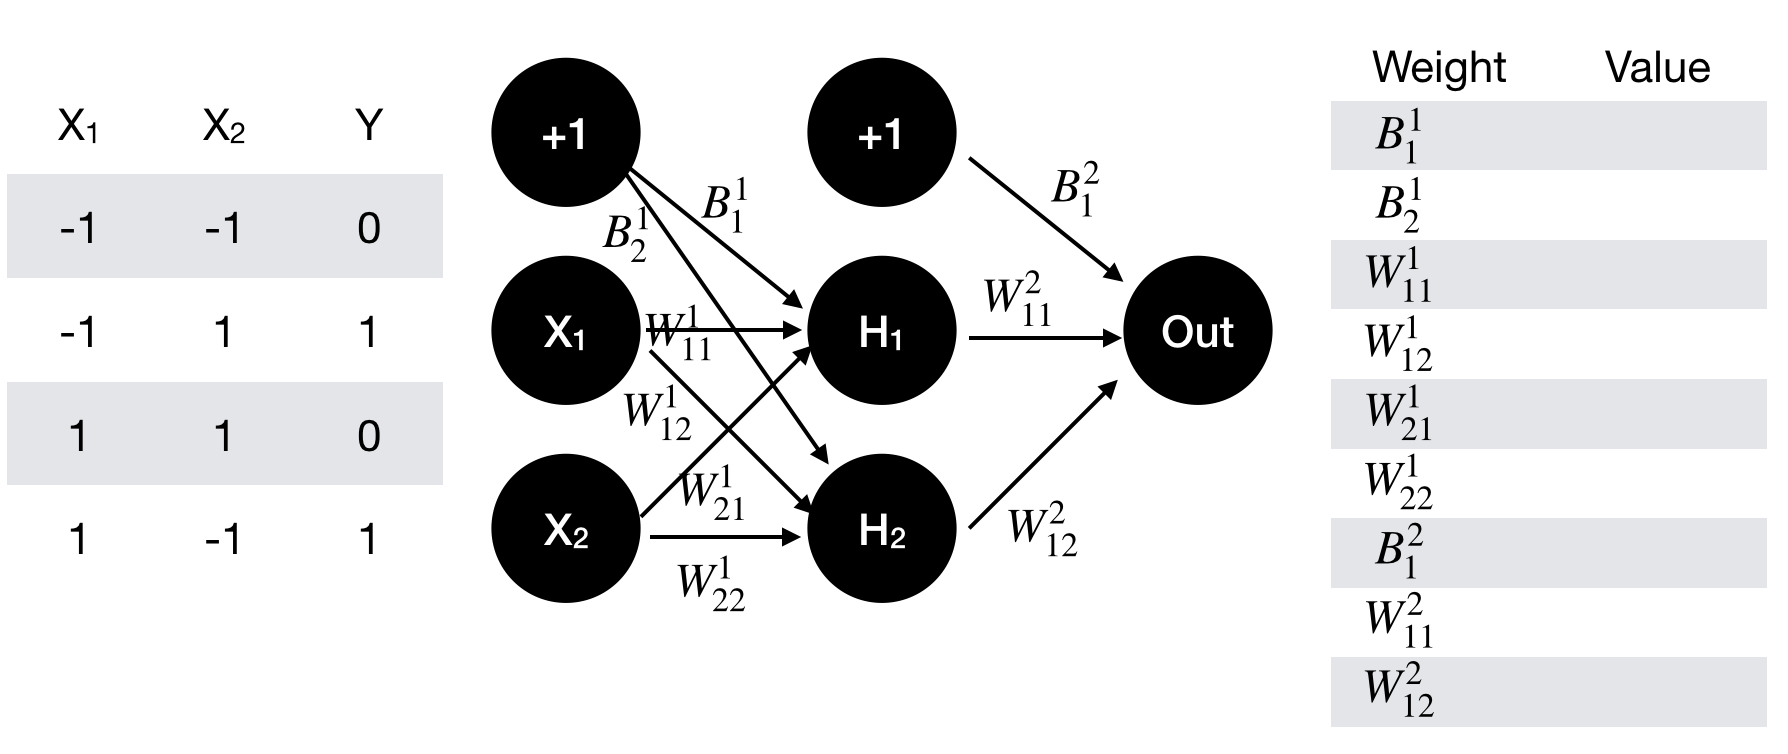
\includegraphics[width=6in]{nn.png}
\end{center}
\begin{solution}
\begin{center}
    \begin{tabular}{|c|c|}
    \hline
        $B^1_1$ & $1$ \\
    \hline
        $B^1_2$ & $1$ \\
    \hline
        $W^1_{11}$ & $-1$ \\
    \hline
        $W^1_{12}$ & $1$ \\
    \hline
        $W^1_{21}$ & $1$ \\
    \hline
        $W^1_{22}$ & $-1$ \\
    \hline
        $B^2_1$ & $1$ \\
    \hline
        $W^2_{11}$ & $-1$ \\
    \hline
        $W^2_{12}$ & $-1$ \\
    \hline
        
    \end{tabular}
\end{center}
% Write your solution here
\end{solution}

\item In this problem, you are going to manually differentiate some simple neural networks. Let $\sigma$ denote the element-wise logistic function. Compute the gradient(s), with respect to each argument, for each of the following functions:
\begin{enumerate}
    \item[(a)] $L(w) = \sigma(w^\top x)$, where $w \in \R^d$
    \item[(b)] $L(w, a) = \sigma(a \cdot \sigma(w^\top x))$, where $w \in \R^d$ and $a \in \R$
    \item[(c)] $L(W, u) = \sigma(u^\top \sigma(W^\top x))$, where $u \in \R^k$ and $W \in \R^{d \times k}$
\end{enumerate}
\begin{solution}
\begin{enumerate}
    \item $\frac{\partial L}{\partial w} = x\sigma(w^\top x)(1 - \sigma(w^\top x))$
    \item $\frac{\partial L}{\partial w} = xa\sigma(a\cdot \sigma(w^\top x))(1 - \sigma(a\cdot \sigma(w^\top x)))\sigma(w^\top x)(1 - \sigma(w^\top x))$ \\
    $\frac{\partial L}{\partial a} = \sigma(a\cdot \sigma(w^\top x))(1 - \sigma(a\cdot \sigma(w^\top x)))\sigma(w^\top x)$
    \item $\frac{\partial L}{\partial W} = xu^\top\sigma(u^\top\sigma(W^\top x))(1 - \sigma(u^\top \sigma(W^\top x)))\sigma(W^\top x)(1 - \sigma(W^\top x))$ \\
    $\frac{\partial L}{\partial u} = \sigma(u^\top\sigma(W^\top x))(1 - \sigma(u^\top \sigma(W^\top x)))\sigma(W^\top x)$
\end{enumerate}
% Write your solution here
\end{solution}


\item In this problem, you will be building {\em neural networks} for digit classification using two different approaches. You will again use the MNIST dataset you have used in past homeworks. If you don't already have them, first go and download the train, validation, and test sets from the class website. (For a description of the data format, please see the last problem of Homework 0). Because your neural network will learn its own feature representation, you will be using the raw image vector as input, $x$. 

You are given two skeleton files: \textit{nn\_models.py}, in which you will define your network network models, and \textit{nn\_main.py} in which you will train and test your networks. {\bf Please append your final code for this problem to the end of your PDF submission.}

\begin{enumerate}

\item[(a)] First, implement a simple multilayer perceptron (MLP) with 1 hidden layer and a logistic activation function. Specifically, your network will have 2 layers: a hidden layer of size $k$ and the final output layer. Remember that your input is of size 28*28=784. Evaluate the training and validation loss at each iteration, that is, average the loss over all batches in each epoch and record the averaged loss value. Do early stopping based on the best validation loss computed in this fashion. For example, if you run 50 epochs, you'll have 50  validation losses, return the model with the lowest validation loss across all epochs and use it to do testing. Plot your training and validation loss curves and report the best test accuracy after experimenting with optimization parameters for gradient descent, as well as the width of your hidden layer. Complete \textit{TODO 1-3} first and then \textit{TODO 4-6} specified in the two given skeleton files. [Hint: You'll either need to save your model during training based on the validation loss and load the best model to return for testing OR you'll need to compute test accuracy after each epoch. Either way of finding the test accuracy for the epoch with best validation loss is fine.]

\item[(b)] 

Convolution is a general concept that appears across many different disciplines. Convolution operators can process many types of data including images, audio, text and other signals. We will see how 2D convolutional neural nets operate for images and try to gain intuition for their various parameterizations.   

2D convolutional neural nets are specified by various hyperparameters, a receptive field (filter size, or kernel size), number of filters $K$, stride $S$, amount of zero padding $P$, and type of pooling. We will represent our input data, as well as the hidden layers, as 3D-arrays. We will denote their dimensions by tuples, WxHxD, of width, height, and depth respectively. Since MNIST images are black-and-white and thus have scalar-valued pixels, the depth of the input image is 1. This means the total input dimensionality is 28x28x1. Suppose, for now, that MNIST was, in fact, in color (RGB). This means the depth of the input image would be 3. Calculate the dimensionality of the output for the following convolutions applied to a color-valued MNIST input:
\begin{enumerate}
\item Convolution Filter size of 2x2, number of filters 33, stride of 2, padding of 0
\item Convolution Filter size of 3x3, number of filters 55, stride of 1, padding of 1
\item Convolution Filter size of 3x3, number of filters 77, stride of 1, padding of 1. Followed by a Max Pooling with filter size of 2x2 and stride 2. 
\end{enumerate}

\item[(c)] For each question above, compute the total number of parameters in the corresponding convolution layer. 

\item[(d)] Now, let's implement a convolutional neural network and use it for digit classification on MNIST. Start with a simple model with one convolutional layer consisting of a 5x5 kernel with 10 filters, a stride of 1, and zero-padding of size 2. Use $\tanh$ as your non-linear activation. Use softmax as the final layer of your model to determine output digit probabilities. Use early stopping as in (a) and report train and validation curves along with your best test accuracy. Complete \textit{TODO 7-8} first and then \textit{TODO 9-11}.

\item[(e)] Finally try experimenting and building deeper architectures (with more layers). You have the option of adding convolution, max-pooling, and fully connected (FC) layers, as well as a choice of activation function for each layer, along with all of the hyper parameters we have discussed so far. To help get started, it maybe easiest to begin by adding convolution and pooling layers that preserve the dimensions of their input, or half them. This should help getting your first deep architectures running without errors. Describe the architecture you found with the best accuracy on the test set. What factors do you find help improve the network? More layers, larger kernel size, different activation function, different optimization methods?

\end{enumerate}
\begin{solution}
% Write your solution here
\end{solution}

\end{enumerate}

\end{document}

